% !TeX root = ../../../book.tex
\section{涉及集合的证明}\label{sec:section3.9}

现在我们已经了解了许多定义和示例,为了介绍什么是集合以及如何操作它们,让我们实际写一些关于集合的严格的、数学上正确的、良好撰写的\textbf{证明}。这里包含的所有命题/引理都是有用的事实,我们可以稍后引用,并且我们希望你能够证明这些主张。(注:引理只是一个需要一些证明的小结果,稍后可以引用来证明更重要的定理。)此外,所有这些证明都具有将来期望你也能提供的质量和严谨性,不久的将来……如果你愿意,可以用此作为指导!

% !TeX root = ../../../book.tex
\subsection{逻辑且严谨:使用定义}

这里要强调的一点是,当我们从描述性的、``冗长的''和直观的证明过渡到更严格的、数学上正确的和正式撰写的证明时,\textbf{正规定义非常重要}。从根本上讲,它们是必不可少的,因为当我们说``$A \cup B$''时,我们需要知道你确切地知道该符号的含义以及它如何在集合 $A$ 和 $B$ 上运行。

另一个例子,当我们说``证明 $A = B$''时,我们心中有一个非常具体的目标,并且你需要跟我们保持一致。对主要概念有直观理解总是有帮助的---``哦,陈述 $A = B$ 只是意味着 $A$ 和 $B$ 具有相同的元素''---但这\emph{不是}我们想要在严格证明中使用的语言/想法。为了证明 $A = B$ 这样的命题,我们需要\textbf{诉诸}集合上下文中``$=$''的\textbf{定义}:$A = B$ 当且仅当 $A \subseteq B$ 且 $B \subseteq A$。

这就是我们说的``满足定义"或``诉诸定义"的含义:要证明某个数学对象具有某种属性,你必须证明该对象满足该属性的正式定义。如果你不熟悉该定义,或者忘记了如何准确地表述它……无论如何,都应该去了解它!我们知道到需要吸收大量新信息,并且当你对某事还不熟悉时,忘记某些地方也在所难免。通过这样做,你将开始更快、更牢固地消化吸收这些想法。

在下面的示例中,你将看到我们如何使用 ``$\subseteq$''、``$=$'' 和 ``$\cap$'' 等定义。对于每个命题/引理,我们最终都会撰写一个正式的证明,但我们也会写出如何\emph{提出这样一个证明}的内容。通常这才是困难的部分!我们认为你会注意到,其中许多解释只是回忆相关定义并思考它的含义以及它在给定情况下应该如何应用。某种程度上,这就是数学。我们只是让我们使用的定义变得越来越复杂。


% !TeX root = ../../../book.tex
\subsection{证明``$\subseteq$''}

回顾子集的定义,后续讨论中将频繁使用:

\begin{definition}
    给定集合 $A$ 和 $B$,若 $A$ 的每个元素也是 $B$ 的元素,则称 $A$ 是 $B$ 的\dotuline{子集}。
\end{definition}

\clearpage

假设需要证明如下命题:
\begin{center}
    设 $A$ 为集合……,$B$ 为集合……,证明 $A \subseteq B$。
\end{center}
如何利用子集的定义进行证明?直观理解是验证``$A$ 的每个元素也是 $B$ 的元素'',但不可仅凭此断言作为结论。关键在于严格证明 $A$ 的任意元素必然属于 $B$。此时``\textbf{任意固定}''这一表述将发挥重要作用。

\subsubsection*{``任意固定''}

如何同时处理 $A$ 的\emph{所有元素}?若 $A$ 仅有有限个元素(如 $3$ 个),或可逐项验证;但当 $A$ 含 $100$ 个、$100$ 万个乃至\emph{无穷}多个元素时,如何系统性地完成证明?

解决方案是引入 $A$ 的一个\textbf{任意固定}元素。其\textbf{任意性}体现在:除属于 $A$ 外,不附加任何特殊假设;其\textbf{固定性}表现为:赋予该元素特定名称(如 $a$, $x$, $t$),并在后续证明中始终指向同一对象。若能证明此元素属于 $B$,即同时证得 $A$ 的\emph{所有}元素均属于 $B$。

\subsubsection*{示例}

让我们通过具体案例理解上述过程。以下展示命题陈述、证明思路分析及正式证明。

\begin{lemma}\label{lemma3.9.1}
    设 $A,B,X$ 为任意集合。若 $X \subseteq A$ 且 $X \subseteq B$,则 $X \subseteq A \cap B$。
\end{lemma}

\emph{直观理解}:通过维恩 (Venn) 图分析。$X \subseteq A$ 与 $X \subseteq B$ 同时成立时,$X$ 必然完全位于 $A$ 与 $B$ 的重叠区域内,即 $A \cap B$ 所表示的区域。这佐证了命题的正确性,但并非严格证明!
\begin{center}
    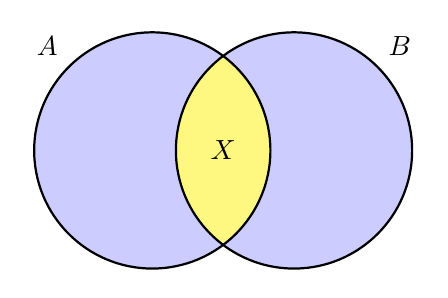
\begin{tikzpicture}[thick, set/.style = {circle, minimum size = 3cm, fill=blue!20}]

        % Set A
        \node[set,label={135:$A$}] (A) at (0,0) {};

        % Set B
        \node[set,label={45:$B$}] (B) at (1.8,0) {};

        % Intersection
        \begin{scope}
            \clip (0,0) circle(1.5cm);
            \clip (1.8,0) circle(1.5cm);
            \fill[yellow!50](0,0) circle(1.5cm);
        \end{scope}

        % Circles outline
        \draw (0,0) circle(1.5cm);
        \draw (1.8,0) circle(1.5cm);

        % Set intersection label
        \node at (0.9,0) {$X$};
    \end{tikzpicture} 
\end{center}

为了证明这个命题,我们引入任意固定元素 $x \in X$。关于它我们知道什么?假设 $X \subseteq A$。符号``$\subseteq$''的定义表明 $X$ 的所有元素都属于 $A$。既然 $x$ 是 $X$ 的元素,那么 $x$ 也属于 $A$。这很方便!类似地,由 $X \subseteq B$ 可得 $x \in B$。综上,我们利用``$\cap$''的定义推知 $x \in A \cap B$。很好!现在将其形式化。

\begin{proof}
    设 $x \in X$ 为任意固定元素。

    假设 $X \subseteq A$,根据 $\subseteq$ 的定义,可得 $x \in A$。

    同理,由 $X \subseteq B$,可得 $x \in B$。

    因为 $x \in A$ 且 $x \in B$,根据 $\cap$ 的定义,这意味着 $x \in A \cap B$。

    综上,对任意 $x \in X$ 均有 $x \in A \cap B$。由于 $x \in X$ 是任意的,因此 $X \subseteq A \cap B$。
\end{proof}

下面看一个稍复杂的例子。

\begin{proposition}
    设 $A$ 和 $B$ 为任意集合。则 $\mathcal{P}(A) \cap \mathcal{P}(B) \subseteq \mathcal{P}(A \cap B)$。
\end{proposition}

这成立吗?回顾 \ref{sec:section3.5} 节习题 \ref{exc:exercises3.5.6} 中的具体示例可知,该命题具有一般性。下面证明其正确性。

\emph{直观理解}:此命题涉及多层次的定义,尤其需注意幂集运算。关键点在于理解 $\mathcal{P}(A)$ 是 $A$ 的所有子集的集合。待证子集关系表明:无论 $\mathcal{P}(A) \cap \mathcal{P}(B)$ 的具体形式如何(稍后分析,但眼下你需要意识到它是一个集合),它都是 $\mathcal{P}(A \cap B)$ 的子集。这一观察将引导后续证明的框架。

无需显式计算 $\mathcal{P}(A) \cap \mathcal{P}(B)$,证明可从``设 $X \in \mathcal{P}(A) \cap \mathcal{P}(B)$ 为任意集合''开始。因为根据``$\subseteq$''的定义,需要证明该集合的任意元素也属于 $\mathcal{P}(A \cap B)$。这确定了证明的\textbf{结构}。

元素 $X \in \mathcal{P}(A) \cap \mathcal{P}(B)$ 是什么?它是集合,且同时属于 $\mathcal{P}(A)$ 和 $\mathcal{P}(B)$。下面直接给出正式证明,但建议你先尝试自行证明。完成后可与下文比较,检验步骤的完整性和表述的清晰性。

\begin{proof}
    设 $X \in \mathcal{P}(A) \cap \mathcal{P}(B)$ 为任意固定集合。

    根据 $\cap$ 的定义,有 $X \in \mathcal{P}(A)$ 且 $X \in \mathcal{P}(B)$。

    因为 $X \in \mathcal{P}(A)$,根据幂集的定义,可知 $X \subseteq A$。

    同理,因为 $X \in \mathcal{P}(B)$ 可知 $X \subseteq B$。

    因为 $X \subseteq A$ 且 $X \subseteq B$,由引理 \ref{lemma3.9.1} 可得 $X \subseteq A \cap B$。

    因为 $X \subseteq A \cap B$,根据幂集的定义,可得 $X \in \mathcal{P}(A \cap B)$。

    由于 $X$ 是任意固定集合,因此可得 $\mathcal{P}(A) \cap \mathcal{P}(B) \subseteq \mathcal{P}(A \cap B)$。
\end{proof}

你的证明与上述一致吗?是否引用了前述引理?或无意中复证了已有结论?请记住:证明的重要价值在于结论的可复用性!虽在证明中复证先前结论无技术错误,但直接引用可节省精力。若解题时产生``似曾相识''的感觉,不妨回溯相关定理或引理,利用已有结论提升效率。


% !TeX root = ../../../book.tex
\subsection{证明``$=$''}

\subsubsection*{双重包含证明}

我们需要再次回顾在集合上下文中``$=$''的定义,因为后续会频繁使用它。

\begin{definition}
    集合 $A$ 和 $B$ 相等,记作 $A = B$,当且仅当 $A \subseteq B$ 且 $B \subseteq A$。
\end{definition}

这一定义完全基于先前定义的``$\subseteq$''(因为``$\supseteq$''的定义等价)。因此,它并非新技术,而是先前技术的重复应用。具体而言,要证明 $A = B$,只需使用上一小节的技术证明 $A \subseteq B$,再证明 $B \subseteq A$。

事实上,这项技术非常常见,因此有专门的名称:\textbf{双重包含}。当证明两个集合彼此是子集并由此得出它们相等时,称为\textbf{双重包含证明}。

\subsubsection*{示例}

让我们看一下双重包含技术的实际应用案例。

\begin{lemma}
    设 $A$ 和 $B$ 为任意集合,则 $A - (A \cap B) = A - B$。
\end{lemma}

\emph{直观理解}:虽然维恩图可以帮助理解这一事实,但它不能替代证明。我们将采用双重包含证明。取元素 $x \in A - (A \cap B)$ 时,可依次应用``$-$''和``$\cap$''的定义,推导出 $x \in A - B$。类似地,取 $y \in A - B$ 时,应用定义可得出 $y \in A - (A \cap B)$。建议读者先尝试自行证明,再参考以下证明过程。

\begin{proof}
    通过双重包含证明 $A - (A \cap B) = A - B$。

    (``$\subseteq$'')设 $x \in A - (A \cap B)$ 为任意固定元素。根据差集定义,$x \in A$ 且 $x \notin A \cap B$。这意味着 $x$ 不可能同时属于 $A$ 和 $B$。已知 $x \in A$,故 $x \notin B$。因此,$x \in A$ 且 $x \notin B$,由差集定义得 $x \in A-B$。这表明 $A - (A \cap B) \subseteq A - B$。

    (``$\supseteq$'')设 $y \in A - B$ 为任意固定元素。根据差集定义,$y \in A$ 且 $y \notin B$。由于 $y \notin B$,$y$ 不可能同时属于 $A$ 和 $B$。由交集定义,$y \notin A \cap B$。结合 $y \in A$ 和 $y \notin A \cap B$,得 $y \in A - (A \cap B)$。这表明 $A - B \subseteq A - (A \cap B)$。

    综上,利用双重包含证明,$A - (A \cap B) = A - B$ 得证。
\end{proof}

纵观上述证明的整体结构,我们看到它分为两部分,因为它是一个双重包含证明。我们\emph{友好地提前}向读者指出了这一点,并将这两个部分明确分开。从技术上讲,忽略这一提示直接深入证明是可行的,但这可能会令读者感到困惑。证明的全部意义在于\emph{使他人信服}你所理解的事实,因此应尽可能让读者轻松理解你的思路。

现在看另一个证明集合相等的例子。这个例子有所不同,因为双重包含的一部分利用了补集操作。作为预习,请思考为何命题 $A \subseteq B$ 与 $\overline{B} \subseteq \overline{A}$ 是\emph{等价的}(假设存在全集 $U$ 满足 $A, B \subseteq U$)。尝试绘制维恩图、举例或直接证明。

\begin{proposition}
    \[\Big\{x \in \mathbb{N} \mid x + \frac{8}{x} \le 6\Big\} = \{2, 3, 4\}\]
\end{proposition}

\begin{proof}
    设 $A = \Big\{x \in \mathbb{N} \mid x + \frac{8}{x} \le 6\Big\}$, $B = \{2, 3, 4\}$。要证明 $A = B$,需要证明 $A \subseteq B$ 且 $B \subseteq A$。

    首先证明 $B \subseteq A$。逐一验证 $B$ 的元素是否满足 $A$ 的不等式:
    \begin{align*}
        2 + \frac{8}{2} &= 6 \le 6 \\
        3 + \frac{8}{3} &= \frac{17}{3} \le 6 \\
        4 + \frac{8}{4} &= 6 \le 6
    \end{align*}
    因为 $2,3,4 \in \mathbb{N}$,我们推导出 $2,3,4 \in A$,从而 $B \subseteq A$。

    接着证明 $A \subseteq B$。我们将证明 $\overline{B} \subseteq \overline{A}$,其中补集以 $\mathbb{N}$ 为全集。也就是说,我们要证明自然数 $1,5,6,7,\dots$ \dotuline{不}属于 $A$。

    为此,验证这些元素均\dotuline{不}满足 $A$ 的不等式定义:

    前两种情况很容易验证:
    \begin{align*}
        1 + \frac{8}{1} &= 9 \nleq 6 \\
        5 + \frac{8}{5} &= \frac{33}{5} \nleq 6
    \end{align*}

    对于其他情况,取任意固定元素 $x \in \mathbb{N}$ 且 $x \ge 6$,有 $x + \frac{8}{x} \ge 6 + \frac{8}{x}$。由于 $\frac{8}{x} > 0$,故 $x + \frac{8}{x} > 6$。

    这表明只有 $2,3,4$ 满足 $A$ 的不等式定义。

    综上,利用双重包含证明,$A = B$ 得证。
\end{proof}

思考为何证明后半部分的方法有效。(这是条件命题的\textbf{逆否}形式,后续章节讨论逻辑时将详细说明。)

让我们来看另一个证明集合相等的例子。这个例子略有不同,因为我们要证明某个集合是空集,为此需要证明它不包含任何元素。

\begin{proposition}
    对于每个 $n \in \mathbb{N}$,定义 $S_n = \mathbb{N}-[n]$。则
    \[\bigcap_{n \in \mathbb{N}}S_n = \varnothing\]
\end{proposition}

如果不理解上面等式的含义,建议尝试几个例子。例如,查看集合 $S_1$、$S_1 \cap S_2$、$S_1 \cap S_2 \cap S_3$ 的元素等等。可以先找出 $\bigcap_{n \in \mathbb{N}}S_n$ 的候选元素,再解释为什么它不属于该集合。之后尝试写出一个正式的证明;可以参考下面的证明过程!

\begin{proof}
    设 $T = \bigcap_{n \in \mathbb{N}}S_n$ 以便后续引用。

    要证明 $T = \varnothing$,需要证明 $T$ 不包含任何元素。注意 $T$ 是多个自然数集合的交集,因此其元素只能是自然数。

    考虑任意固定元素 $x \in \mathbb{N}$,我们需要证明 $x \notin T$。

    已知 $x \in [x] = \{1,2,\dots, X\}$,因此根据``$-$''的定义,$x \notin \mathbb{N}-[x]$。

    根据定义,$T$ 的元素必须属于每个 $\mathbb{N} - [n]$ 形式的集合。我们已经(至少)确定了交集中的一个集合 $\mathbb{N} - [x]$,使得 $x$ 不属于该集合。因此,$x$ 不可能是 $T$ 的元素,因为它不属于所有此类集合,所以 $x \notin T$。

    因为 $x \in \mathbb{N}$ 是任意的,我们证明了 $T$ 的元素中不包含自然数,故 $T$ 为空集。
\end{proof}

\emph{总结}:让我们再解释一下这个证明方法为何有效。我们证明了 $T$ 中没有元素,即 $T \subseteq \varnothing$。这就完成了论证,因为 $\varnothing \subseteq T$ 对任何集合恒成立。因此双重包含论证的条件已满足,可以得出 $T = \varnothing$ 的结论。

让我们再举一个例子。这个例子为我们提供了练习索引集操作的机会,本节习题中还有许多类似问题,我们鼓励你尽可能多尝试解答!

\begin{proposition}
    对于每个 $n \in \mathbb{N}$,定义 $A_n = \{x \in \mathbb{R} \mid 0 \le x < \frac{1}{n}\}$。则
    \[\bigcap_{n \in \mathbb{N}}A_n = \{0\}\]
\end{proposition}

思考上述命题的含义:在数轴上画出 $A_n$ 的图示,交集符号``$\cap$''表示什么?为什么 $0$ 属于该交集?为什么它是\emph{唯一}的元素?

证明的关键在于``$\cap$''的定义,请特别注意\emph{对于每个}这一条件:

\begin{definition}
    由集合 $I$ 索引的一系列集合 $A_i$ 的交集为
    \[\bigcap_{i \in I} A_i = \{x \in U \mid x \in A_i \text{\ 对于每个\ } i \in I\}\]
    其中我们假设存在集合 $U$ 满足对于每个 $i \in I, A_i \subseteq U$。
\end{definition}

请牢记:索引交集由属于所有成分集合的元素构成。因此在证明中,我们需要说明:
\begin{enumerate}[label=(\arabic*)]
    \item $0$ 确实是所有 $A_n$ 集合的元素。
    \item 不存在其他实数满足此性质,即对于任意非零实数,总存在某个 $A_n$ 不包含该数。
\end{enumerate} 

\begin{proof}
    首先,我们来证明
    \[\{0\} \subseteq \bigcap_{n \in \mathbb{N}}A_n\]

    这需要证明对于每个 $n \in \mathbb{N}, 0 \in A_n$。

    设 $n \in \mathbb{N}$ 为任意固定元素。注意,不等式 $0 \le 0 \le \frac{1}{n}$ 必然成立。

    (注:可能有人会担忧,因为``在极限内'' $0$ 是否``同时''小于每个分数 $\frac{1}{n}$,但这不是重点!正确的思路是:$0 \in A_1$ 吗?是的,因为 $0 \le 0 < 1$。$0 \in A_2$ 吗?是的,因为 $0 \le 0 < \frac{1}{2}$。$0 \in A_3$ 吗?是的,因为 $0 \le 0 < \frac{1}{3}$。依此类推。该不等式对于每个 $n \in N$ 均成立,所以 $0$ 是每个此类集合的元素。如果你不担心这一点,可跳过此备注,继续前进!)

    因此,对于每个 $n \in \mathbb{N}, 0 \in A_n$,所以根据 ``$\cap$'' 的定义,$\displaystyle{0 \in \bigcap_{n \in \mathbb{N}} A_n}$。这就证明了 $\displaystyle{\{0\} \subseteq \bigcap_{n \in \mathbb{N}} A_n}$。

    接着,我们来证明
    \[\bigcap_{n \in \mathbb{N}}A_n \subseteq \{0\}\]

    考虑在全集 $\mathbb{R}$ 下这些集合的\dotuline{补集}。具体来说,我们将证明
    \[\overline{\{0\}} \subseteq \overline{\bigcap_{n \in \mathbb{N}}A_n}\]

    这意味着我们要证明每个非零实数\dotuline{不属于}某个 $A_n$。

    设 $x \in \mathbb{R}$ 为任意固定元素,且 $x \ne 0$。也就是说,要么 $x > 0$ 要么 $x < 0$。接下来分两种情况讨论:

    \begin{itemize}
        \item 情况 1:假设 $x > 0$。考虑实数 $\frac{1}{x} \in \mathbb{R}$。由于 $\mathbb{R}$ 中的自然数集无上界,因此存在 $M \in \mathbb{N}$ 满足 $M > \frac{1}{x}$。
        
        (注意:思考为什么会这样。我们尚未\dotuline{证明} $\mathbb{N}$ 是无限的,即数字沿着实数轴``永远延续下去'',但我们希望这些想法对你来说直观且合理。)

        取 $M \in \mathbb{N}$ 且 $M > \frac{1}{x}$。由于 $x > 0$,不等式两边同时乘以 $x$;由于 $M > 0$(因此 $\frac{1}{M} > 0$),不等式两边再次乘以 $\frac{1}{M}$。由此可得 $x > \frac{1}{M}$。由于 $A_M$ 要求 $-\frac{1}{M} < x < \frac{1}{M}$,因此 $x \ne A_M$。

        由于 $x \notin A_M$,所以 $x$ 肯定不是所有此类集合的元素。因此
        \[x \notin \bigcap_{n \in \mathbb{N}} A_n\]

        \item 情况 2:假设 $x < 0$。考虑 $-x > 0$。采用与上面相同的逻辑,必然存在 $M \in \mathbb{N}$ 满足 $M > \frac{1}{-x} = -\frac{1}{x}$。整理不等式可得 $x < -\frac{1}{M}$。所以 $x \notin A_M$,因此 
        \[x \notin \bigcap_{n \in \mathbb{N}} A_n\]
    \end{itemize}

    综上,我们已经证明,任意 $x \in \mathbb{R}$ 且 $x \ne 0$ 不属于至少一个 $A_n$,因此任何这样的 $x$ 都不是它们交集的元素。因此,由双重包含论证可得:
    \[\{0\} = \bigcap_{n \in \mathbb{N}} A_n\]
\end{proof}

该证明具有一定难度,建议反复阅读确保理解每个步骤。特别留意选择 $M \in \mathbb{N}$ 且满足 $M > \frac{1}{x}$ 的动机:这并凭借直觉神奇偶得,而是从目标 $x > \frac{1}{M}$ 反推不等式得到的。


% !TeX root = ../../../book.tex
\subsection{证伪}

\subsubsection*{举个例子}

考虑如下命题:
\begin{center}
    对于任意集合 $F, G, H$,如果 $F \subseteq G \cup H$,则要么 $F \subseteq G$ 要么 $F \subseteq H$。
\end{center}

这种说法成立吗?如果成立,我们该如何证明呢?我们取任意固定元素 $x \in F$。由于 $F \subseteq G \cup H$,这告诉我们 $x \in G \cup H$。 相应地,$x \in G$ 或 $x \in H$。这都没错吧?我们的证明完成了吗?

我们希望你能看出来这是行不通的!特别是,我们最后还没有满足 ``$\subseteq$'' 的定义。如果我们的目标是证明 ``$F \subseteq G$ 或 $F \subseteq H$'',那么我们应该得出结论,其中一个或另一个成立:即 $F$ 的\emph{每个}元素都是 $G$ 的元素,或者 $F$ 的\emph{每个}元素都是 $H$ 的元素。

我们发现 $F$ 的每个元素本身要么是 $G$ 的元素,要么是 $H$ 的元素,但我们不能确定 $F$ 的所有元素都是 $G$ 的元素或都是 $H$ 的元素。再次通读最后两段,以确保你跟上了逻辑。可能很容易为这个命题写出一个``证据'',却没有意识到你迈出了错误的一步!

\subsubsection*{定位错误}

这种对错误的识别是我们要发展的技能之一,它将在多个方面提供帮助。你会注意到,许多练习(到目前为止有一些,但随着我们继续深入,会有更多)要求你找出某些主张``证明''中的缺陷。通过指出存在缺陷,从而帮助你获得正确的证明(或多个证明,视情况而定)。阅读在逻辑、事实和清晰度上有误的证明是一项基本技能。更重要的是,仔细阅读别人的成果必然会让你成为一个对自己的成果更加挑剔的读者,并且会帮助你发现像前面段落中那样的潜在错误。如果你没有抓住它,请不要担心;既然你已经看到了它,你将来就会留意类似的错误!正如我们所说,这项技能是不断发展起来的,到读完本书时,你将成为数学证明的出色读者和作者。

\subsubsection*{反例}

那么,现在我们该怎么办?我们刚刚意识到我们上面的``证明''不起作用。这是否意味着该说法实际上是错误的?实际上,这一切意味着(到目前为止)我们的证明尝试失败了。也许其他一些逻辑路线会神奇地把我们带到难以捉摸的结论。

或者,也许这个说法确实是错误的。我们怎样才能证明这一点?考虑一下该命题的逻辑形式:它说某些陈述对于任意集合 $F,G,H$ 都成立。它说假设 $F \subseteq G \cup H$ 总是必然意味着 $F \subseteq G$ 或 $F \subseteq H$。要证明这并不总是成立,我们只需要找到所谓的\textbf{反例}即可。

我们将在下一章形式化逻辑时再次讨论所有这些想法,但现在你需要知道的是:\textbf{反例}是一个具体的、详细的、描述性的例子,它说明了关于``每个……''或``任意……''或``皆可能……''实际上并\emph{不}适用于所有情况。反例相当于通过展示该类中\emph{不具有}该属性的一个对象来\textbf{反驳}整个类对象具有某种属性的陈述。

\subsubsection*{示例}

让我们看一下寻找和陈述反例的过程如何解决我们上面的例子。\\

\begin{example}
    对于任意集合 $F, G, H$,如果 $F \subseteq G \cup H$,则要么 $F \subseteq G$ 要么 $F \subseteq H$。
\end{example}

这个命题应该适用于任意集合 $F,G,H$,因此当我们描述反例时,我们最好\emph{准确地}描述这三个集合是什么。我们不能只是解释解决这个问题的方法并讨论如何可能存在具有特定属性的三个集合。我们必须通过明确定义它们来告诉读者它们到底是什么。这就是我们反驳这一主张的第一行,但我们不能直接跳到这一点,因为我们还不知道如何定义它们!

这就是工作或乐趣所在:我们需要尝试这些集合所需的属性来帮助我们想出一个例子。回想一下,我们希望这些集合满足某些属性:我们应该确保假设 $F \subseteq G \cup H$ 成立,但我们希望结论 --- $F \subseteq G$ 或 $F \subseteq H$ --- 为假。

这是意味着什么呢?好吧,我们认为你会同意,从逻辑上讲,该陈述的``相反''或``否定''是 ``$F \nsubseteq G$'' 和 ``$F \nsubseteq H$''。(\textbf{逻辑否定}的概念将在下一章中再次出现;目前,我们认为你可以通过应用指导日常生活的逻辑原则来理解它。很快,我们将正式化这一想法。)

我们现在有一个具体的目标:找到满足以下所有三个条件的三个集合 $F,G,H$:

\begin{align*}
    F &\subseteq G \cup H \\
    F &\nsubseteq G \\
    F &\nsubseteq H \\
\end{align*}

接下来需要考虑的一件事是 ``$\nsubseteq$'' 的含义。我们有 ``$\subseteq$'' 的定义,那么它的``相反''或``否定''是什么?为了使 $F \subseteq G$ 成立,我们要求 $F$ 的每个元素也是 $G$ 的元素;因此,如果不成立,那么 $F$ 中至少有一个元素不是 $G$ 的元素。同理也适用于 $F \nsubseteq H$。现在,我们可以通过应用定义以一种有用的方式重申我们的目标:

\begin{align*}
    &F \text{的每个元素都是} G \text{的元素或} H \text{的元素} \\
    &F \text{中至少有一个元素不是} G \text{的元素} \\
    &F \text{中至少有一个元素不是} H \text{的元素} \\
\end{align*}
这对于最终找到我们的反例非常有帮助!我们总结了声明的所有基本部分,并以更直观的方式重述了这些属性。剩下的工作就是在草稿纸上写写画画,看看我们能想出什么。一种方法是为 $F, G$ 和 $H$ 及其潜在的``重叠''绘制一种``空''维恩图,然后填充足够的元素以满足上述三个属性。

第一个条件要求集合 $F$ 完全``位于'' $G$ 和 $H$ 之内;但是,第二个和第三个条件要求存在 $F$ 的两个元素,其中一个不是 $G$ 的元素,另一个不是 $H$ 的元素。这就是我们要做的!你可能会说这是一个简单的例子,但我们说这是一个\emph{有效的}例子。现在让我们开始写下我们的反驳:

\begin{proof}
    下面声明为假:
    \begin{center}
        对于任意集合 $F, G, H$,如果 $F \subseteq G \cup H$,则要么 $F \subseteq G$ 要么 $F \subseteq H$。
    \end{center}
    我们将用反例来反驳该观点。

    定义 $F = \{1, 2\}, G = \{1\}, H = \{2\}$。

    请注意 $G \cup H = \{1, 2\}$。由于 $F = G \cup H$,那么当然 $F \subseteq G \cup H$。因此,该主张的假设成立。

    然而,请注意 $2 \in F$ 但 $2 \notin G$。因此,$F \nsubseteq G$。

    同样,请注意 $1 \in F$ 但 $1 \notin H$。因此,$F \nsubseteq H$。

    因此,该主张为假。
\end{proof}

该示例的一个重要教训如下:

\begin{center}
    寻找反例不一定是最有趣或最复杂的,你也不需要以某种方式描述所有可能的反例。我们只需要找到一个反例,我们需要看看它是如何运作的。
\end{center}

就是这样!这正是我们在上面的证明中所做的:我们定义了所有重要的对象(三个集合 $F,G,H$),然后指出并描述了它们具有的所有相关属性。我们并没有让读者检查反例是否有效;我们向他们展示了细节。我们并没有争论宇宙中某个地方存在这样的集合;我们只是认为宇宙中存在这样的集合。我们明确地定义了它们。

这很重要,我们希望你的反例具有与我们上面类似的证明结构。当你尝试给出反例时,大部分工作将在证明开始之前``在幕后''进行。不过,一旦你找到了反例,就像我们一样把它写出来。


% !TeX root = ../../../book.tex
\subsection{习题}

\subsubsection*{温故知新}

以口头或书面的形式简要回答以下问题。这些问题全都基于你刚刚阅读的内容,所以如果忘记了具体的定义、概念或示例,可以回去重读相关部分。确保在继续学习之前能够自信地回答这些问题,这将有助于你的理解和记忆!

\begin{enumerate}[label=(\arabic*)]
    \item $\subseteq$ 的定义是什么?我们如何用它来证明 $A \subseteq B$?
    \item 两个集合相等意味着什么?
    \item 什么是\emph{双重包含}证明?
    \item 什么是反例?
    \item 假设 $A,B,U$ 是集合,且 $A,B \subseteq U$。为什么我们可以通过证明 $\overline{B} \subseteq \overline{A}$ 来证明 $A \subseteq B$ 呢?尝试说服朋友相信这是一种有效的技术。
\end{enumerate}

\subsubsection*{小试牛刀}

尝试回答以下问题。这些题目要求你实际动笔写下答案,或(对朋友/同学)口头陈述答案。目的是帮助你练习使用新的概念、定义和符号。题目都比较简单,确保能够解决这些问题将对你大有帮助!

\begin{enumerate}[label=(\arabic*)]
    \item 首先,\textbf{证明}如下声明:
        \begin{center}
            对于任意集合 $A,B,C$,子集关系 $A - (B - C) \subseteq (A - B) \cup C$ 成立。
        \end{center}
        接着,找到这些集合实际上总是\emph{相等}这一主张的\emph{反例}。
    \item 假设 $A,B,C$ 是集合并且 $A \subseteq B$。证明 $A \times C \subseteq B \times C$。
    \item 假设 $A \subseteq C$ 且 $B \subseteq D$。证明 $A \times C \subseteq B \times C$。
    \item 设 $A = \{x \in \mathbb{R} \mid x^2 > 2x + 8\}$ 且 $B = \{x \in \mathbb{R} \mid x > 4\}$。对于以下每个主张,要么证明它是正确的,要么提供反例来证明它是错误的。
        \begin{enumerate}[label=(\alph*)]
            \item $A \subseteq B$
            \item $B \subseteq A$
        \end{enumerate}
    \item 设 $A, B, U$ 为集合,且 $A, B \subseteq U$。通过\emph{双包含论证}证明 $A - B = A \cap \overline{B}$。
    \item 令 $S = \{x \in \mathbb{R} \mid -2 < x < 5\}$ 且 $T = \{x \in \mathbb{R} \mid -4 \le x \le 3\}$。在 $\mathbb{R}$ 作为全集的情况下,$S \cap \overline{T}$ 是什么?找到一个集合,然后使用双包含论证证明它是正确的。
    \item \textbf{证明}以下断言:如果 $A \subseteq B$,则 $\mathcal{P}(A) \subseteq \mathcal{P}(B)$。\label{exc:exercises3.9.7}
    \item 对于每个 $n \in \mathbb{N}$ 令 $S_n = \{x \in \mathbb{R} \mid -\frac{1}{n} < x < \frac{1}{n}\}$。证明
        \[\bigcap_{n \in \mathbb{N}}S_n = \{0\}\]
    \item 设 $I = \{x \in \mathbb{R} \mid 0 < x < 1\}$。对于每个 $x \in I$,定义 $S_x = \{y \in \mathbb{R} \mid x < y < x + 1\}$。 证明
        \[\bigcup_{x \in I}S_x = \{z \in \mathbb{R} \mid 0 < z < 2\}\]
    \item 对于每个 $n \in \mathbb{N}$,定义集合 $A_n$ 和 $B_n$
        \begin{align*}
            A_n &= \Big\{x \in \mathbb{R} \mid 0 ≤ x < \frac{n - 1}{n}\Big\} \\
            B_n &= \Big\{y \in \mathbb{R} \mid -\frac{1}{n} < y < 1\Big\}
        \end{align*}
        通过双重包含论证\textbf{证明}以下集合相等:
        \[\bigcup_{n \in \mathbb{N}}A_n = \bigcap_{n \in \mathbb{N}}B_n\]
\end{enumerate}
